\chapter{Verwandte Arbeiten}
\label{chap:verwarbeiten}

Da in dieser Arbeit verschiedene Forschungsbereiche miteinander kombiniert werden, ist dieses Kapitel in zwei Abschnitte eingeteilt: Es wird mit einigen verwandten Arbeiten im Bereich der Bildsegmentierung begonnen, dabei wird insbesondere auf texturbasiertes Clustering und die Nutzung von neuronalen Netzen eingegangen. Anschließend wird die Analyse der Marsoberfläche, hauptsächlich der Kratererkennung, betrachtet.



\section{Bildsegmentierung}
\label{sec:segmentation}

\subsection{Texturbasiertes Clustering von Bilddateien}
\label{ssec:clustering}

Da die zu analysierenden Aufnahmen der Marsoberfläche nur in Graustufen vorhanden sind, eignet sich eine farbbasierte Clustering-Methode nicht um diese zuverlässig zu clustern. Selbst wenn dieses mit auf die Helligkeitswerte der Eingabedatei angewandt wird, führt dies dazu, dass der Algorithmus das Bild nach den Helligkeitswerten segmentiert, und nicht wie gewünscht anhand ihrer Oberflächenstruktur. So ergibt ein Clustering des Kraters aus \figurename~\ref{fig:ex_crater} durch den SLIC-Algorithmus \cite{achanta_10} das in \figurename~\ref{fig:slic_crater} sichtbare Ergebnis.\footnote{SLIC-Implementierung: \textit{scikit-image}\\Parameter: \textit{compactness}=20, \textit{n\_segments}=30\\Cluster gefüllt mit ihren jeweiligen Durchnittshelligkeitswerten}

\begin{figure}[h!]
	\centering
	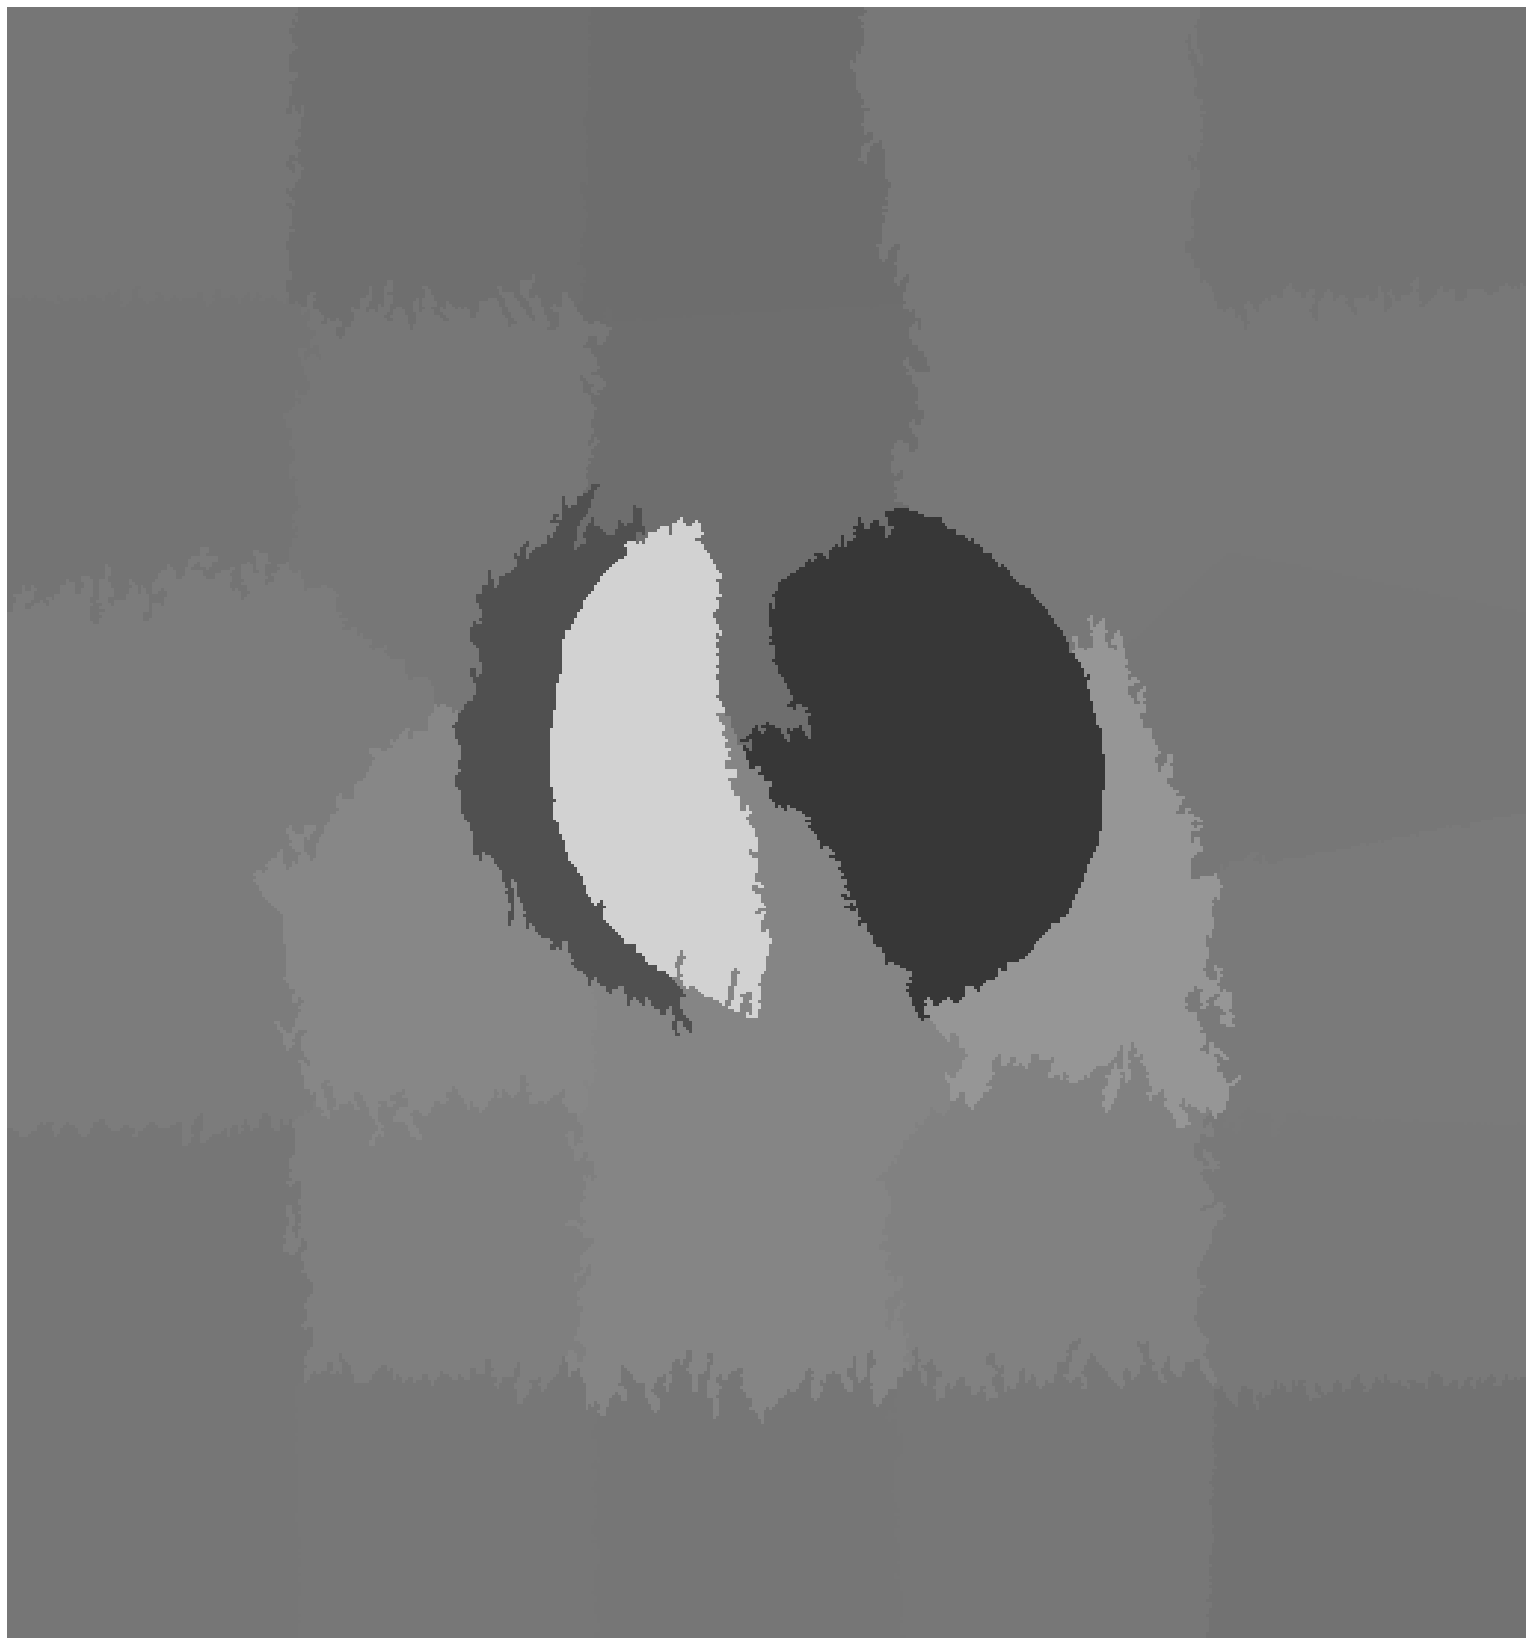
\includegraphics[width=0.35\textwidth,keepaspectratio]{images/gen/GEN_slic_crater.png}
	\captionsetup{format=plain,width=0.35\textwidth}
	\caption{Ergebnis des SLIC-Algorithmus angewandt auf eine Krateraufnahme}
	\label{fig:slic_crater}
\end{figure}

Hier ist erkennbar, dass der Krater in jeweilige Licht- und Schattenregionen (bedingt durch den Lichteinfall im flachen Winkel) unterteilt wird. Dieses Phänomen wird sich zwar in \ref{sec:craterdetection} zu nutze gemacht, ist hier allerdings ungewollt.

Wenn nun der in Unterabschnitt~\ref{ssec:kanezaki} beschriebene Ansatz verfolgt wird, wird das neuronale Netz daraufhin trainiert, eine Aufnahme anhand ihrer Helligkeitsinformationen hin zu trainieren. Da dies nicht gewollt ist, wird statt einem farb-/helligkeitsbasierten Clusteringalgorithmus wie SLIC ein texturbasiertes Clustering genutzt.

Eine geeignete Methode wird in \cite{jain_91} beschrieben: In dieser Methode wird eine Reihe von Gabor-Filtern dazu benutzt, die Textur des Bildes zu analysieren. Dieser Prozess verläuft wie folgt:

Zuerst wird eine reihe von Gabor-Filtern erstellt. Ein Beispiel, welches nach der originalen Ausarbeitung nachgestellt wurde, findet sich in \figurename~\ref{fig:tsugf_filters}. Es gilt zu beachten dass jeder Filter in mehrmals in unterschiedlichen Größen erstellt wird.

\begin{figure}[h!]
	\centering
	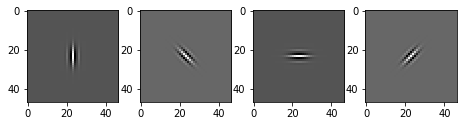
\includegraphics[width=0.5\textwidth,keepaspectratio]{images/gen/GEN_tsugf_filterbank.png}
	\captionsetup{width=0.5\textwidth}
	\caption{Zum texturbasierten Clustering genutze Filterbank}
	\label{fig:tsugf_filters}
\end{figure}

Diese werden anschließend über das in den Unterabschnitten~\ref{ssec:conv} und \ref{ssec:convlayer} beschriebene Konvolutionsverfahren angewandt. Dieser Vorgang resultiert in einem Datenwürfel, bei welchem die ersten beiden Dimensionen gleich der Höhe und breite der Eingabebilddatei sind, und die dritte Dimension gleich der Anzahl der genutzen Filter ist. Somit enthält jede Schicht des Würfels Informationen darüber, wie sehr und wo im Bild das Muster der jeweiligen Filterbank \enquote{erkannt} wird. Dies ist in \figurename~\ref{fig:tsugf_101027_raw} sichtbar.

\begin{figure}[h!]
	\begin{subfigure}[t]{0.32\textwidth}
		\centering
		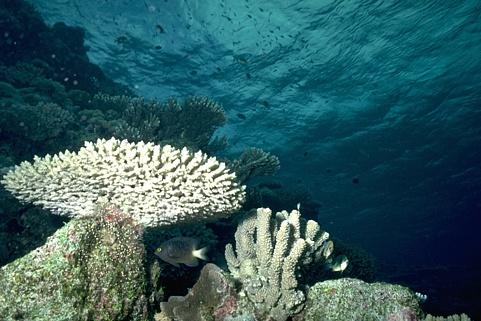
\includegraphics[width=\textwidth,keepaspectratio]{images/bsd/101027.jpg}
		\captionsetup{format=plain}
		\subcaption{}
		\label{fig:bsd_101027}
	\end{subfigure}
	\hfill
	\begin{subfigure}[t]{0.32\textwidth}
		\centering
		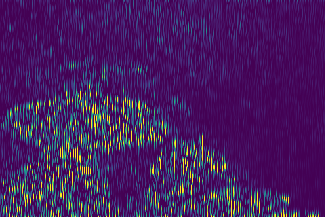
\includegraphics[width=\textwidth,keepaspectratio]{images/gen/GEN_tsugf_filterbank_101027_1.png}
		\subcaption{}
	\end{subfigure}
	\hfill
	\begin{subfigure}[t]{0.32\textwidth}
		\centering
		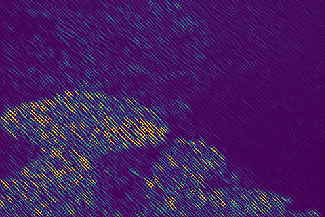
\includegraphics[width=\textwidth,keepaspectratio]{images/gen/GEN_tsugf_filterbank_101027_2.png}
		\subcaption{}
	\end{subfigure}
	\hfill
	\begin{subfigure}[t]{0.32\textwidth}
		\centering
		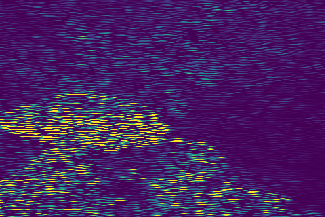
\includegraphics[width=\textwidth,keepaspectratio]{images/gen/GEN_tsugf_filterbank_101027_3.png}
		\subcaption{}
	\end{subfigure}
	\hfill
	\begin{subfigure}[t]{0.32\textwidth}
		\centering
		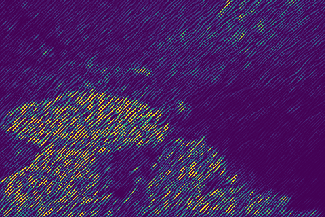
\includegraphics[width=\textwidth,keepaspectratio]{images/gen/GEN_tsugf_filterbank_101027_4.png}
		\subcaption{}
	\end{subfigure}
	\hfill
	\begin{subfigure}[t]{0.32\textwidth}
		\hfill
	\end{subfigure}
	\caption{Ergebnisse (b-e) der Konvolution des Beispielbildes (a, aus \cite{bsd500}) mit den jeweiligen Filtern}
	\label{fig:tsugf_101027_raw}
\end{figure}

Anschließend wird der k-Means-Algorithmus auf diesen Datenwürfel angewandt: Dieser teilt eine beliebige Anzahl von Messpunkten (in diesem Fall je ein Vektor pro Pixel) in eine vorher festgelegte Menge an Clustern ein. Es werden also in dieser Anwendung Messpunkte/Pixel mit ähnlichen Texturen in Cluster zusammengefasst.

In der Praxis sind für die erfolgreiche Anwendung dieser Methode allerdings noch einige Optimierungen notwendig: \cite{mathworks_15}

\begin{itemize}
	\item Weichzeichnung:\\
	Da die Anwendung des Konvolutionsverfahrens wie in \figurename~\ref{fig:tsugf_101027_raw} sichtbar zu einer streifenartigen Merkmalsextraktion führen kann, macht es in vielen Fällen Sinn, die jeweiligen Merkmalsebenen weichzuzeichnen. Als Radius eignet sich hier ein Wert, welcher groß genug ist um die Streifen zu entfernen, aber klein genug ist, als dass die Ränder der jeweiligen erkannten Texturen nicht in benachbarte Texturen überfließen.
	\item Räumlicher Bezug:\\
	Damit diese Cluster eine (bessere) räumliche Beziehung zueinander haben, wird zu den Merkmalsdimensionen je eine Schicht hinzugefügt, welche ausschließlich mit den X-Koordinaten der jeweiligen Pixel gefüllt ist. Selbiges geschieht für die jeweiligen Y-Koordinaten. Da diese vom k-Means Algorithmus auch zusammen geclustert werden, entsteht ein örtlicher Bezug unter den Clustern.
	\item Normalisierung:\\
	Die jeweiligen Schichten sollten vor der Anwendung des k-Means-Algorithmus normalisiert werden um zu vermeiden, dass manche Merkmale stärer gewichtet werden als andere. Dies ist insbesondere wichtig, wenn wie oben genannt die Farb- oder Positionswerte den Merkmalsdimensionen hinzugefügt werden, da diese sich oft auf unterschiedlichen Skalen gegenüber den Konvolutionsergebnissen befinden.
	\item Farbdimensionen:\\
	Wenn die Eingabedatei eine RGB-Aufnahme ist, können diese drei Farbkanäle zur besseren Unterscheidung von unterschiedlichen Clustern mit ähnlichen Texturen genutzt werden. Dazu wird die Aufnahme in ihre drei Farbkanäle aufgeteilt und diese drei Schichten anschließend als Merkmalsdimensionen dem Datenwürfel hinzugefügt.
\end{itemize}

Das schrittweise Hinzufügen dieser Optimierungen ist in \figurename~\ref{fig:tsugf_optim} sichtbar.

\begin{figure}[h!]
	\begin{subfigure}[t]{0.32\textwidth}
		\centering
		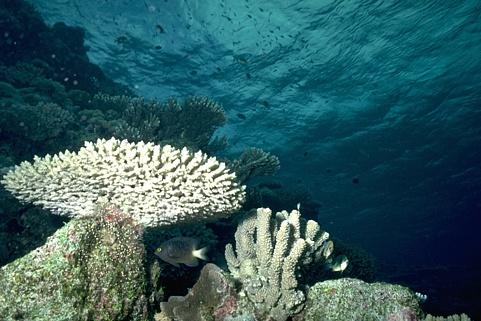
\includegraphics[width=\textwidth,keepaspectratio]{images/bsd/101027.jpg}
		\subcaption{Beispielbild (aus \cite{bsd500})\\\xspace}
	\end{subfigure}
	\hfill
	\begin{subfigure}[t]{0.32\textwidth}
		\centering
		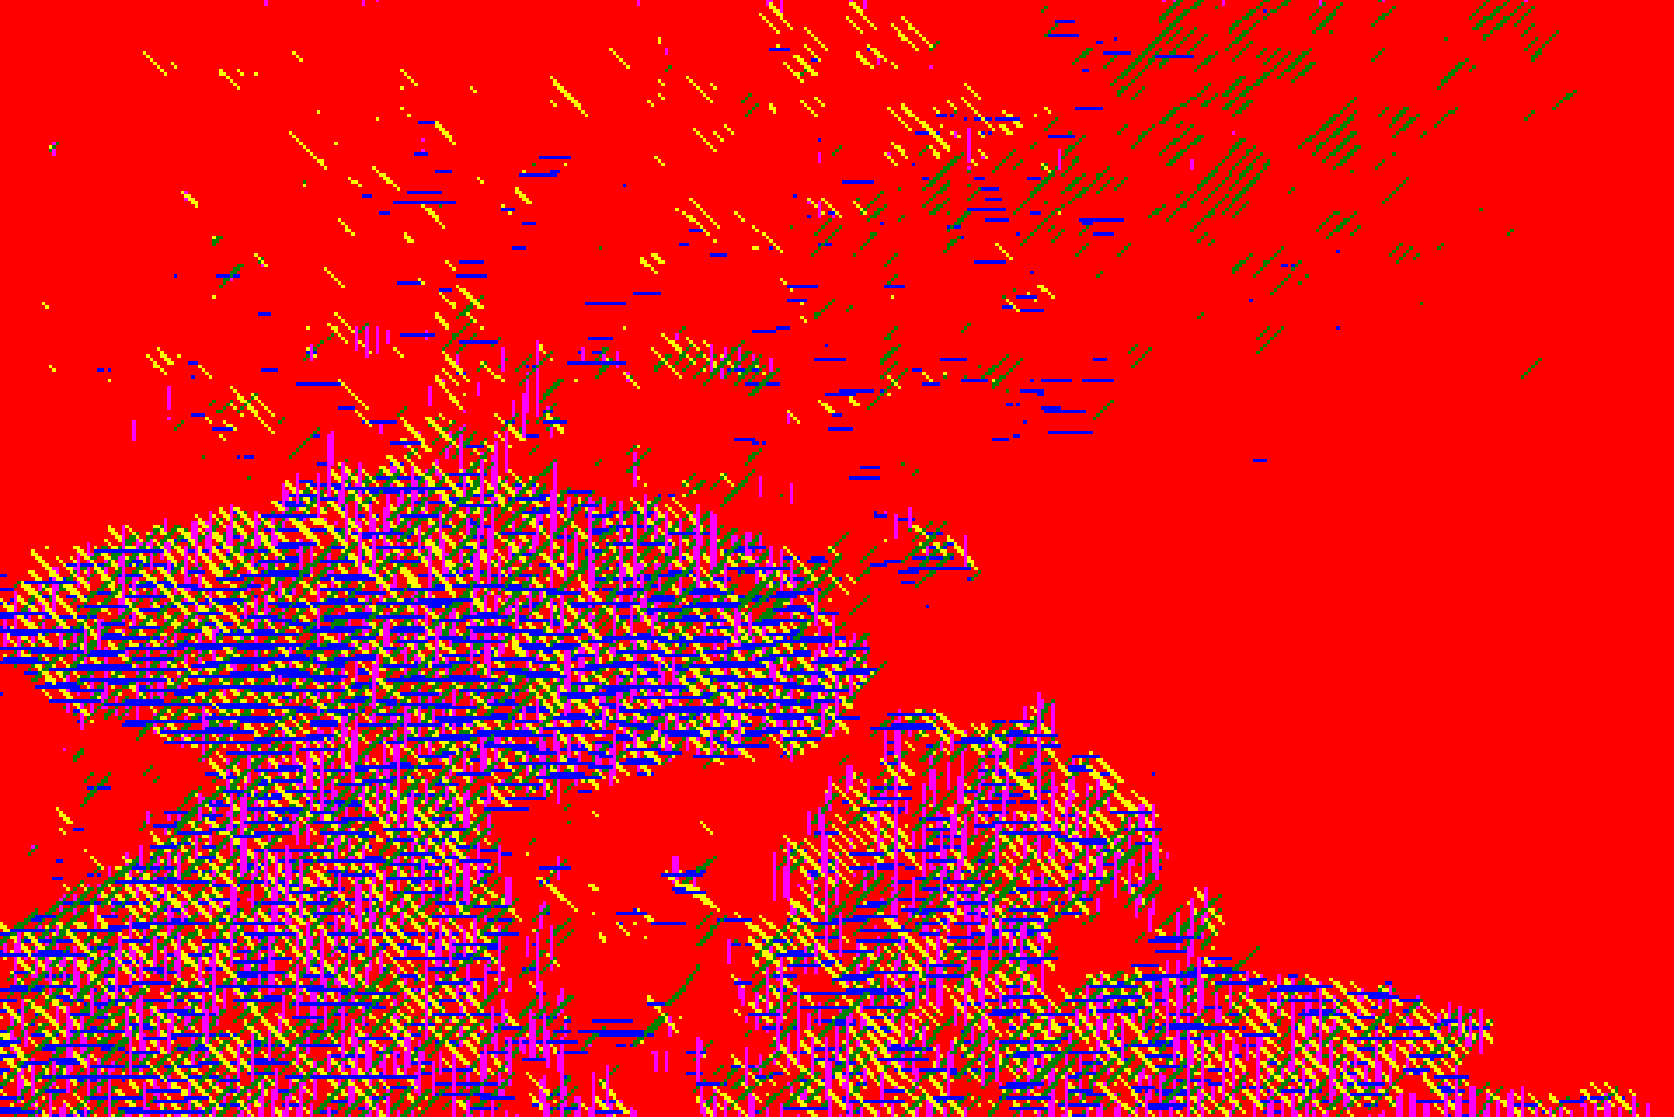
\includegraphics[width=\textwidth,keepaspectratio]{images/gen/GEN_tsugf_filterbank_101027_raw.png}
		\captionsetup{format=plain}
		\subcaption{Originales Clusteringergebnis\\\xspace}
	\end{subfigure}
	\hfill
	\begin{subfigure}[t]{0.32\textwidth}
		\centering
		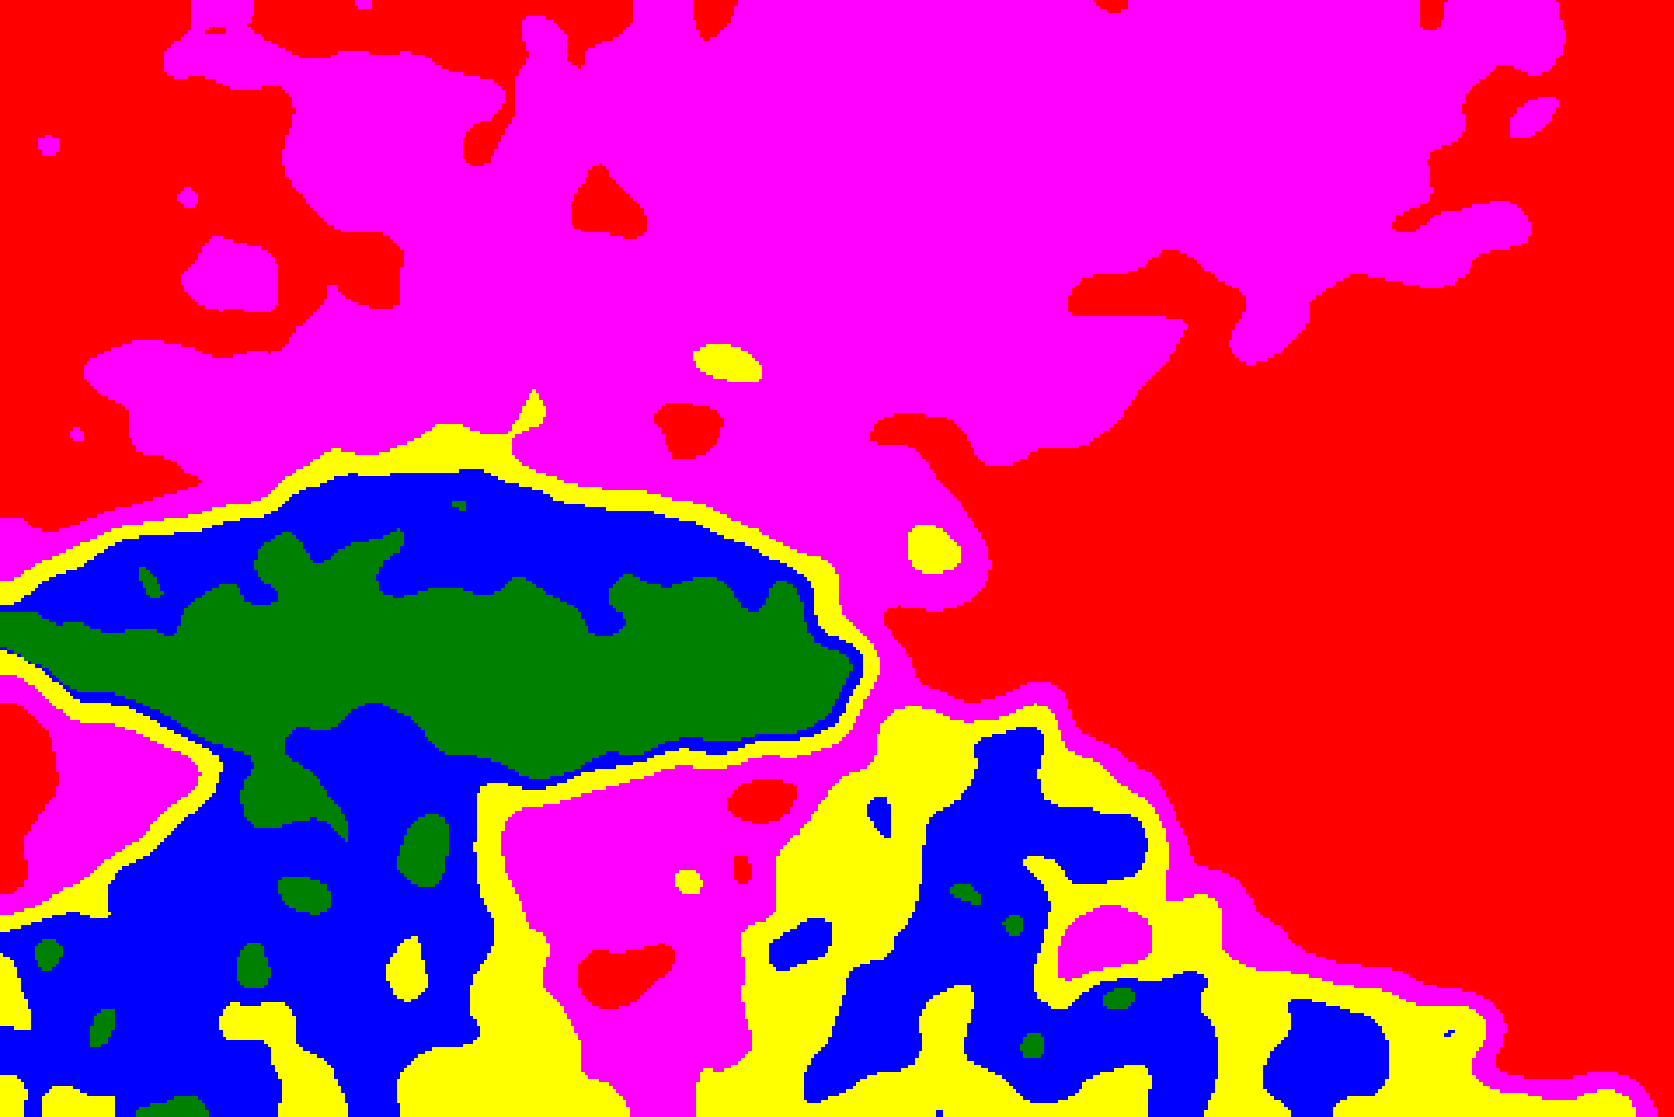
\includegraphics[width=\textwidth,keepaspectratio]{images/gen/GEN_tsugf_filterbank_101027_blur.png}
		\subcaption{Weichzeichnen der Konvolutionsergebnisse}
	\end{subfigure}
	\hfill
	\begin{subfigure}[t]{0.32\textwidth}
		\centering
		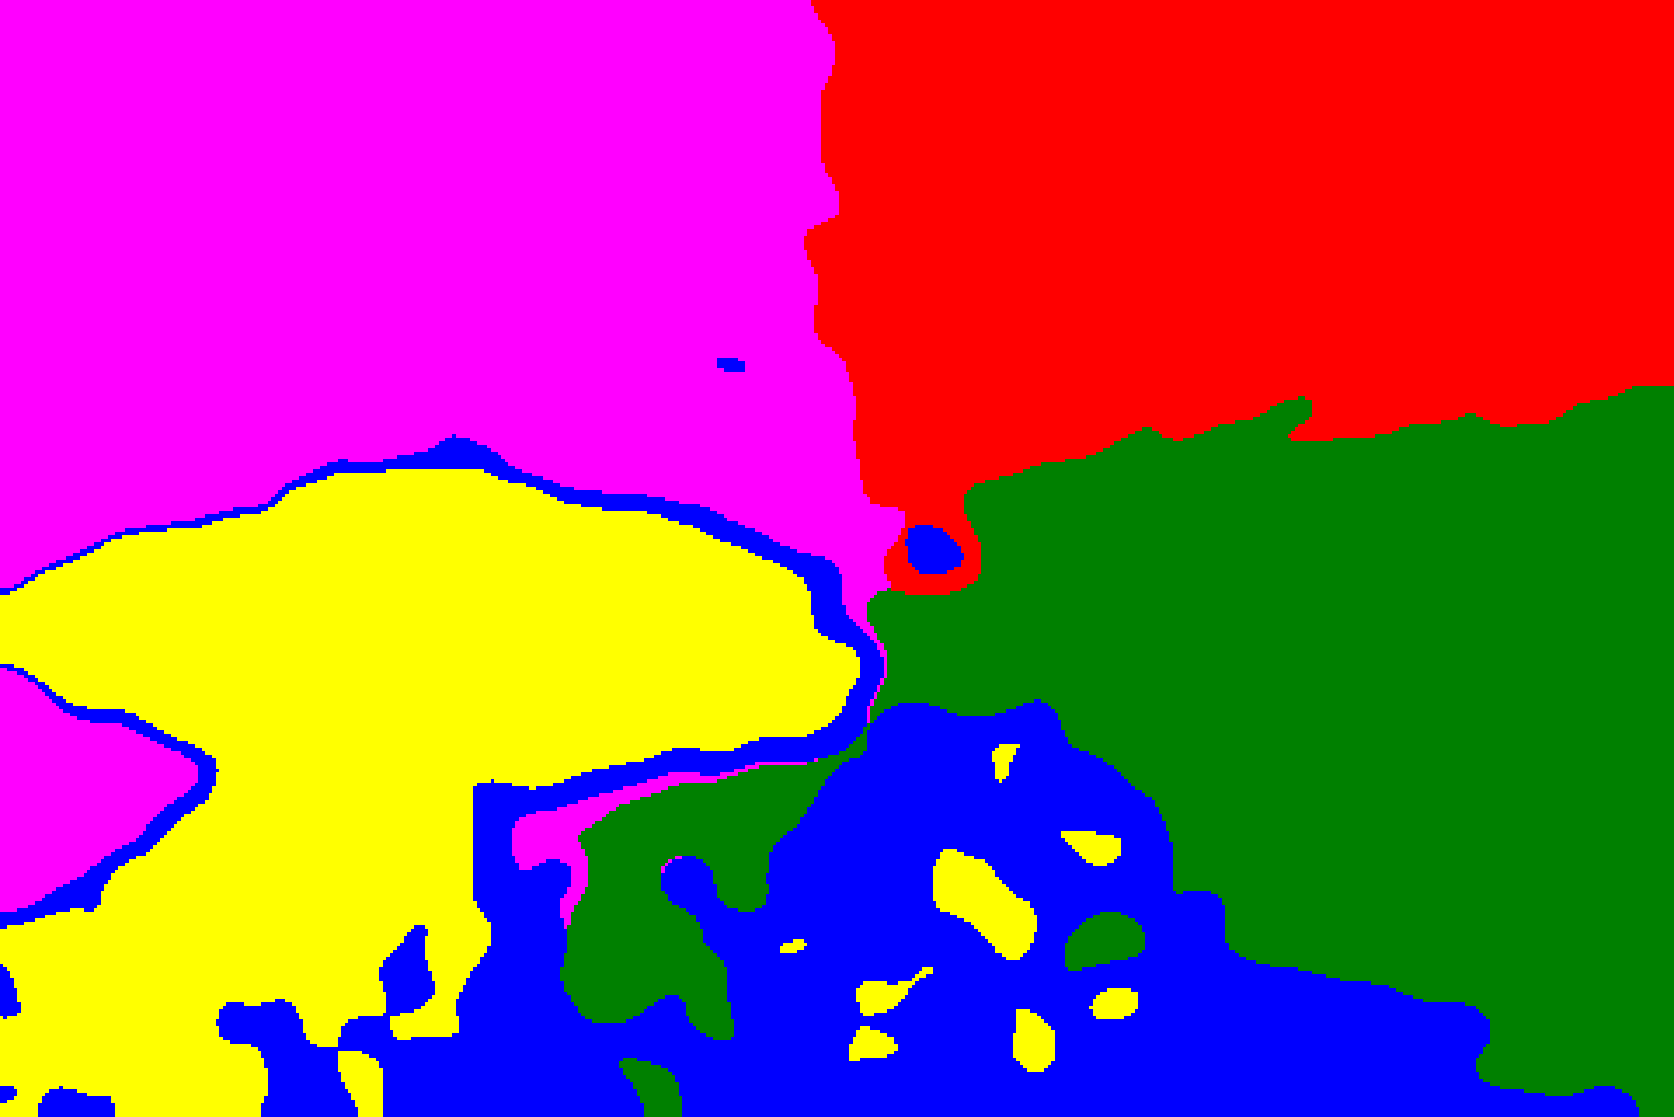
\includegraphics[width=\textwidth,keepaspectratio]{images/gen/GEN_tsugf_filterbank_101027_blur_norm_spatial.png}
		\subcaption{Zusätzliche räumliche Informationen und Normierung}
	\end{subfigure}
	\hfill
	\begin{subfigure}[t]{0.32\textwidth}
		\centering
		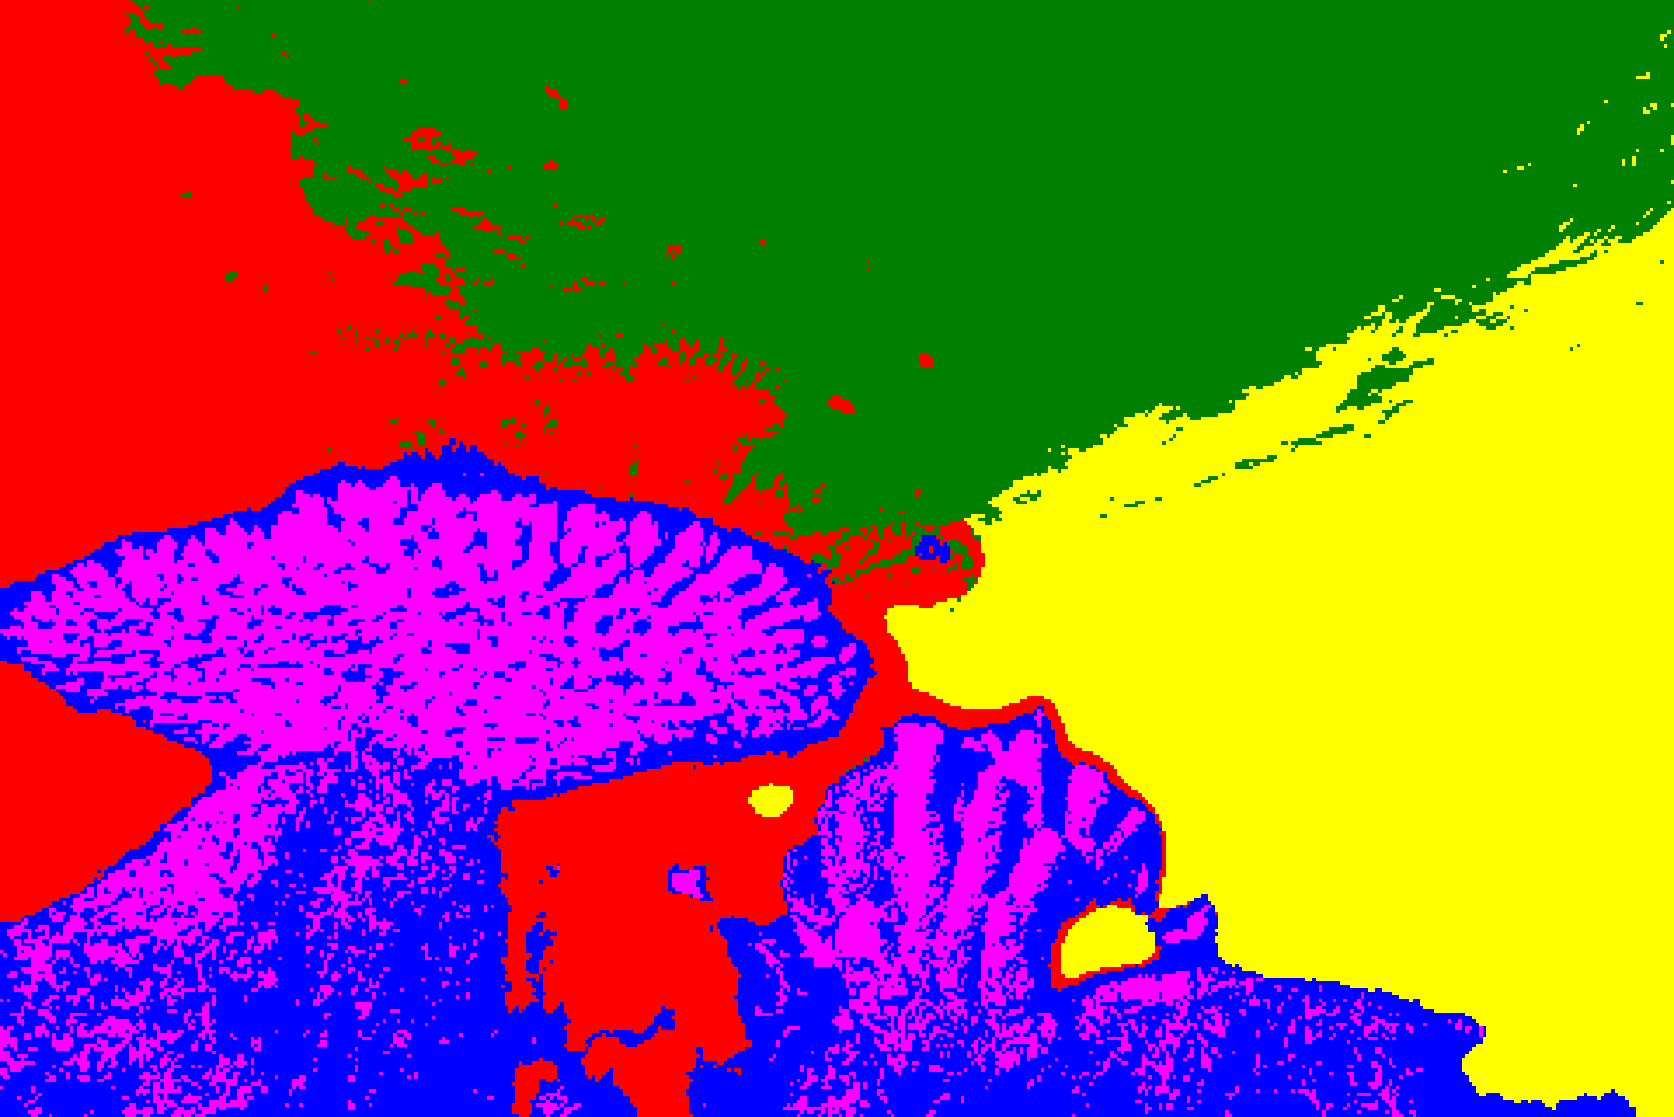
\includegraphics[width=\textwidth,keepaspectratio]{images/gen/GEN_tsugf_filterbank_101027_blur_norm_spatial_color.png}
		\subcaption{Zusätzliche Farbinformationen}
	\end{subfigure}
	\hfill
	\begin{subfigure}[t]{0.32\textwidth}
		\hfill
	\end{subfigure}
	\caption{Optimierung des Clusteringverfahrens}
	\label{fig:tsugf_optim}
\end{figure}

\subsection{Bildsegmentierung ohne Ground Truth durch Backpropagation}
\label{ssec:kanezaki}
In \cite{kanezaki_18} wird ein Ansatz beschrieben, Convolutional Neural Networks zur Bildsegmentierung zu nutzen. Die Besonderheit an diesem Ansatz ist allerdings, dass er nicht wie frühere Versuche CNNs zur Bildsegmentierung zu nutzen auf überwachtem Lernen basiert, sondern unüberwachtes Lernen nutzt.

Dieser Ansatz erstellt eine Mapping-Funktion $c_n=f(x_n)$, die jedem der $N$ $p$-dimensionalen Pixel mit dem Merkmalsvektor $\{x_n\in\mathbb{R}^p\}_{n=1}^N$ eines Eingabebildes ein Clusterlabel $c$ mit $\{c_n\in\mathbb{Z}\}_{n=1}^N$ zuordnet.

Während das Ziel das gleiche wie bei überwachtem Lernen ist, wird hier weder eine Ground Truth, noch ein vorher angelerntes Neuronales Netz benötigt.

Erreicht wird dieses Ziel durch einen iterativen Prozess, in welchem ein anfangs untrainiertes neuronales Netz eine Bildsegmentierung erzeugt, welche anschließend mithilfe einer im Vorhinein erstellten, konstanten Segmentierung optimiert wird. Diese wird in diesem Paper über den SLIC-Algorithmus \cite{achanta_10} erzeugt. Der gesamte Algorithmus ist in \figurename~\ref{fig:Kan18_01} dargestellt. 

\begin{figure}[h!]
	\centering
	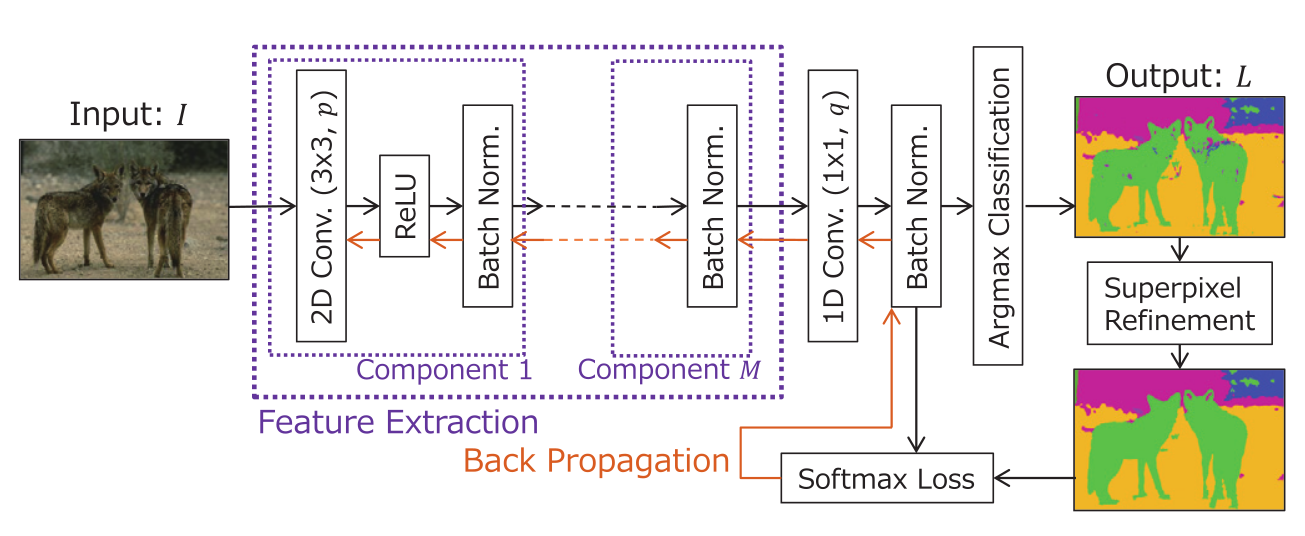
\includegraphics[width=.8\textwidth,keepaspectratio]{images/Kan18_01.png}
	\caption{Vorgehensweise nach Kanezaki, aus \cite{kanezaki_18}}
	\label{fig:Kan18_01}
\end{figure}

Eine vergleichbare, aber weitreichendere Methode --~der DEC Algorithmus~-- wird in \cite{junyuan_16} dargestellt: Auch besteht das Ziel daraus, $N$ Punkte $\{x_n\in X\}_{n=1}^N$ in $k$ verschiedene Cluster mit den jeweiligen Clustermitten $\mu_j, j\in\left[1, k\right]$ einzuteilen. Entgegen des Ansatzes von Kanezaki hingegen wird hier nicht direkt im Merkmalsraum $X$ des Eingabebildes geclustert, stattdessen wird dieser zuerst über eine nichtlineare Funktion $f_\theta: X\rightarrow Z$ in einen Merkmalsraum $Z$ abgebildet. $\theta$ ist dabei ein lernbarer Parameter, sodass das genutzte Neuronale Netz zwei Parameter zeitgleich optimiert: $\theta$, und die Position der Clustermitten $\mu_j$.

Der DEC-Algorithmus besteht aus zwei Phasen:
\begin{enumerate}
	\item Parameterinitialisierung:\\
Um die Startparameter für $\theta$ zu Generieren wird schichtenweise ein Stacked Autoencoder (SAE) schichtenweise aufgebaut. Jede Schicht des SAEs ist ein rauschunterdrückender Autoencoder, welcher wie folgt definiert ist: \cite{junyuan_16}
\begin{eqnarray}
\bar{x}&\sim&Dropout(x)\\
h &=& g_1(W_1\tilde{x}+b_1)\\
\tilde{h} &\sim& Dropout(h)\\
y &=& g_2(W_2\tilde{h}+b_2)
\end{eqnarray}
Zuerst wird Encoder-Decoder-Paar dazu trainiert, ein Signal wiederherzustellen, nachdem dies eine Encoder-Schicht (hier ) durchlaufen hat. Anschließend wird der Parameter $h$ dazu genutzt, ein weiteres Paar zu trainieren (\vgl \figurename~\ref{fig:sae}). Am Ende dieses Lernens besteht $\theta$ aus der Menge aller Gewichtungen $W$ und Bias $b$ der verschiedenen Encoder Schichten. Diese Encoder-Schichten beschreiben nun die Funktion $f_\theta$, welche den originalen Merkmalsraum $X$ des Bildes in den reduzierten Merkmalsraum $Z$ umwandelt.

Die initialen Clustermitten werden durch den k-Means-Algorithmus auf dem Merkmalsraum $Z$ generiert.
	\item Parameteroptimierung
Das eigentliche Lernen des DEC-Algorithmus findet in zwei, sich abwechselnden Phasen statt:

Zuerst wird eine Zuweisung von den Datenpunkten des Merkmalsraumes zu den Koordinaten der Clusterzentren berechnet. Zu diesem Zweck wird eine Wahrscheinlichkeitsverteilung (die $t$-Verteilung) genutzt: Diese berechnet die Wahrscheinlichkeit, dass ein bestimmter Datenpunkt einem bestimmten Cluster zugewiesen wird.

Anschließend werden die Parameter $\theta$ der Funktion $f_\theta$ optimiert. Die zu verringernde Verlustfunktion ist an dieser Stelle die Kullback-Leibler-Divergenz. Somit wird hier eine Wahrscheinlichkeitsfunktion gelernt, welche sich möglichst wenig von der oben beschriebenen, iterativ generierten $t$-Verteilung unterscheidet. Der eigentliche Optimierungsprozess der Clustermitten und der Parameter für $\theta$ findet über das Gradientenverfahren (\vgl Unterabschnitt~\ref{ssec:gradientenverfahren}) statt.
\end{enumerate}

\begin{figure}[h!]
	\centering
	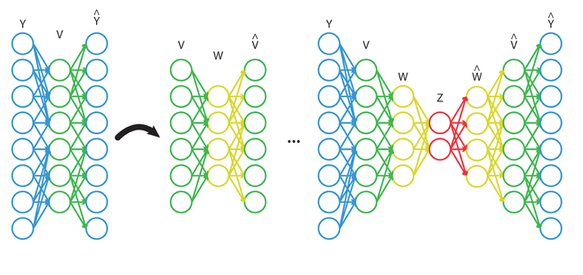
\includegraphics[width=.8\textwidth,keepaspectratio]{images/BK15_01.png}
	\caption{Initialisierung eines Stacked Autoencoders, modifiziert, aus \cite{berniker_15}}
	\label{fig:sae}
\end{figure}

\section{Kratererkennung}
\label{sec:craterdetection}

In \cite{bandeira_10} und dessen Fortsetzung \cite{bandeira_12} wird ein neuer Ansatz zur Kratererkennung vorgestellt. Zuvor wurden diese meist manuell katalogisiert, dies resultierte darin, dass nur die größten Krater dokumentiert wurden, oder darin, dass nur vergleichsweise kleine Bereiche innerhalb eines akzeptablen Zeitraums verarbeitet werden konnten. Daher legen die Autoren insbesondere Wert auf die korrekte Erkennung von kleineren Kratern.

Die erarbeitete Vorgehensweise beginnt damit, dass über einen möglichst effizienten Algorithmus (hier der Algorithmus von Urbach \etal \cite{urbach_stepinski_2009}) eine Vorsortierung von Krater-Kandidaten berechnet wird. Als Alternative zu diesem Algorithmus werden \cite{bandeira_07} und \cite{salamuniccar_10} genannt.

Der genutzte Algorithmus ist zwar relativ effizient, da er parallel alle Merkmale eliminiert, die nicht auf Krater hindeuten. Frühere Algorithmen hingegen griffen meist auf eine Brute-Force-Methode zurück. Zur Erkennung von Krater (\bzw Krater-Kandidaten) wird hier die Tatsache genutzt, dass diese auf Abbildungen meisten aus nebeneinander liegenden, starken Schatten- und Hightlight-Regionen bestehen.

Nach dieser Vorsortierung und Pre-Processing Schritten (in Form von Histogramm-Optimierung) werden in \cite{bandeira_10, bandeira_12} neun Bitmasken (siehe \figurename~\ref{fig:BDS12_01}) in verschiedenen Positionen, Größen und Ausrichtungen über die Kandidaten gelegt. Die Wahrscheinlichkeit, dass der Kandidat ein Krater ist, berechnet sich aus der Übereinstimmung zwischen den Bitmasken und dem eigentlichen Kandidatenbild. Abschließend werden die Ergebnisse mithilfe eines angepassten AdaBoost Algorithmus optimiert. Das Post-Processing besteht aus der Eliminierung von ungewöhnlich geformten Kratern.

\begin{figure}[h!]
	\centering
	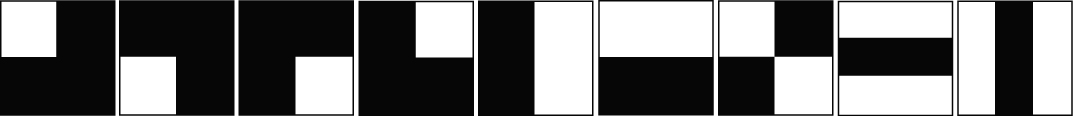
\includegraphics[width=.8\textwidth,keepaspectratio]{images/BDS12_01.png}
	\caption{Die neun, zur Merkmalsextrahierung genutzen Bitmasken, aus \cite{bandeira_12}}
	\label{fig:BDS12_01}
\end{figure}

In \figurename~\ref{fig:BDS12_02} sind die von AdaBoost ausgewählten, am stärksten gewichteten Bitmasken-Überlagerungen dargestellt. Es ist zu beachten, dass der Krater im Hintergrund nur ein Beispiel ist, und nicht alle Krater, die von den jeweiligen Bitmasken überlagert werden, darstellt.

\begin{figure}[h!]
	\centering
	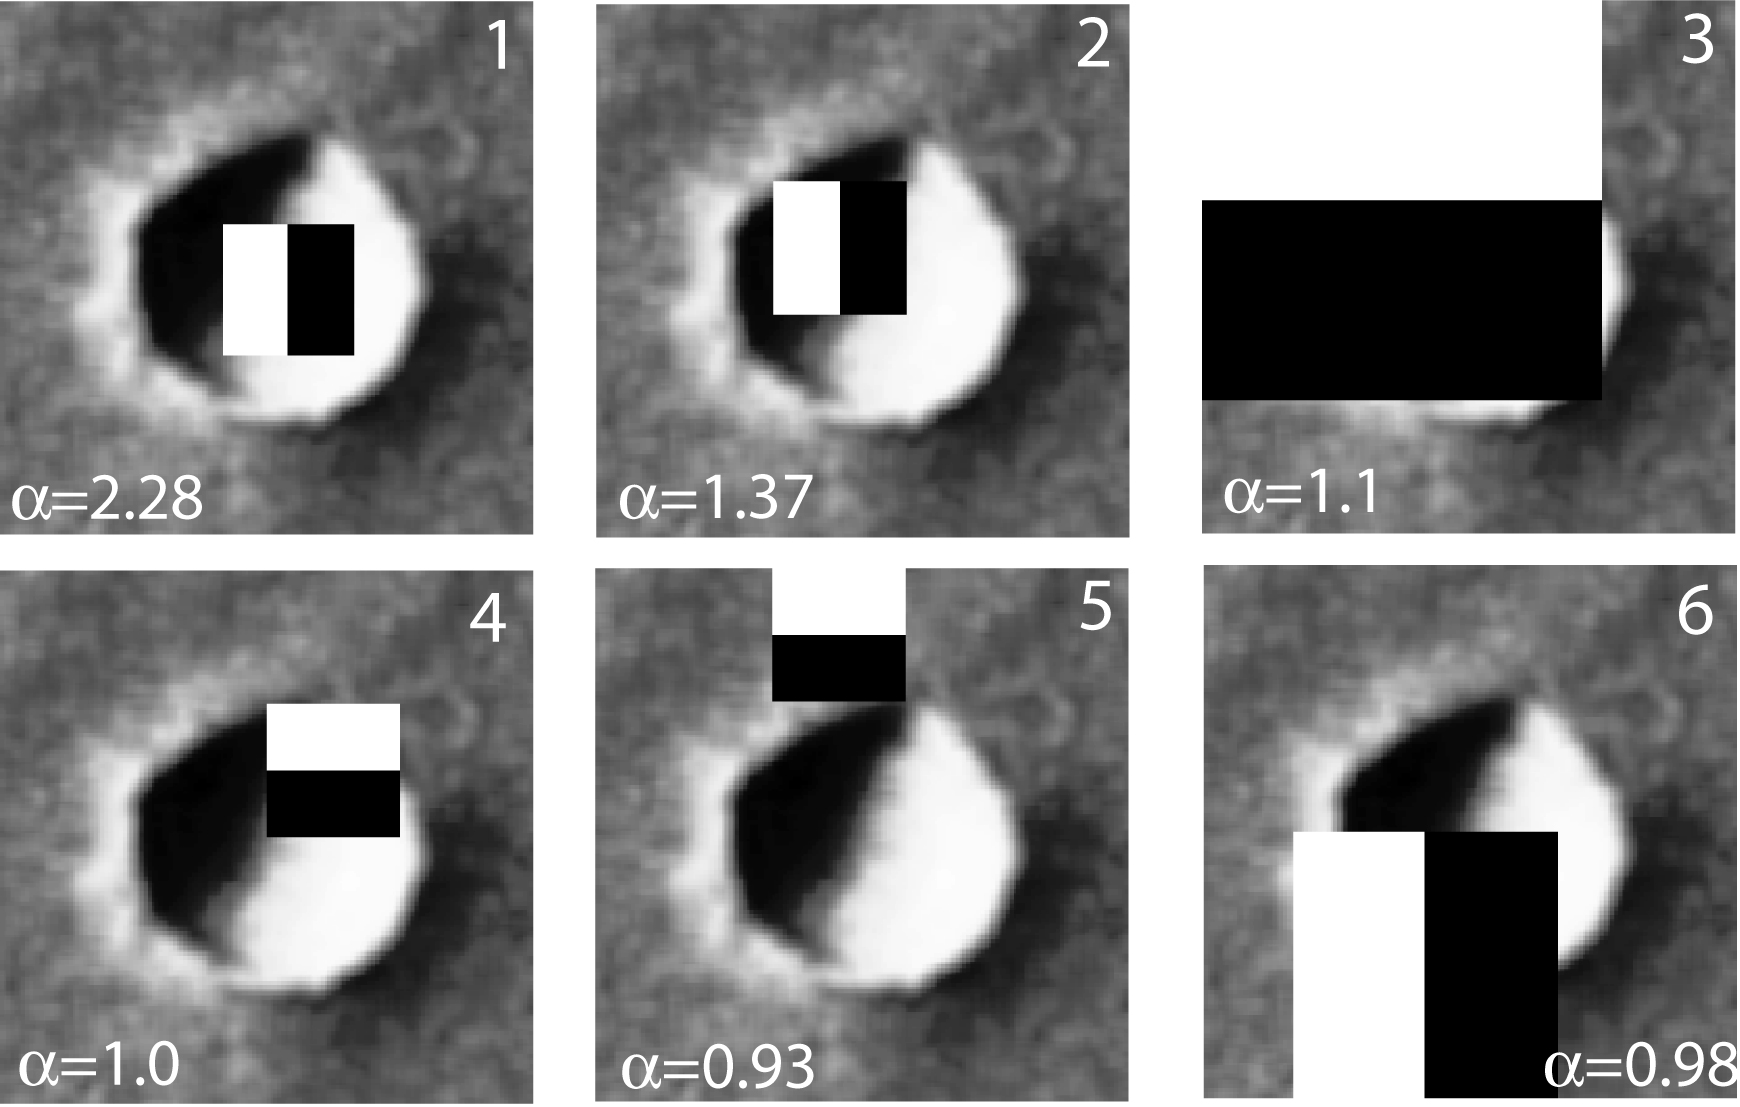
\includegraphics[width=.5\textwidth,keepaspectratio]{images/BDS12_02.png}
	\caption{Die sechs am stärksten gewichteten Bitmasken, aus \cite{bandeira_12}}
	\label{fig:BDS12_02}
\end{figure}

\subsection{Kratererkennung über Neuronale Netze}
\label{ssec:crater_cnn}
Auf der Basis des erwähnten, automatisch generierten Marskrater-Datensatz, wird in \cite{cohen_16} ein neuronales Netzwerk daraufhin trainiert, selbst unterscheiden zu können, ob ein Kraterkandidat auch wirklich ein Krater ist. Die Architektur des Netzwerkes ist in \figurename~\ref{fig:CLLD16_01} zu sehen. Zur Evaluierung der Ergebnisse wird hier das 10-fache Kreuzvalidierungsverfahren genutzt. Dies bedeutet, dass der Eingabedatensatz zehn-geteilt wird, und jeweils neun Teile zum trainieren und ein Teil zum Evaluieren genutzt wird. Das Ergebnis ist der Durchschnitt der jeweiligen F1-Scores.

\begin{figure}[H]
	\centering
	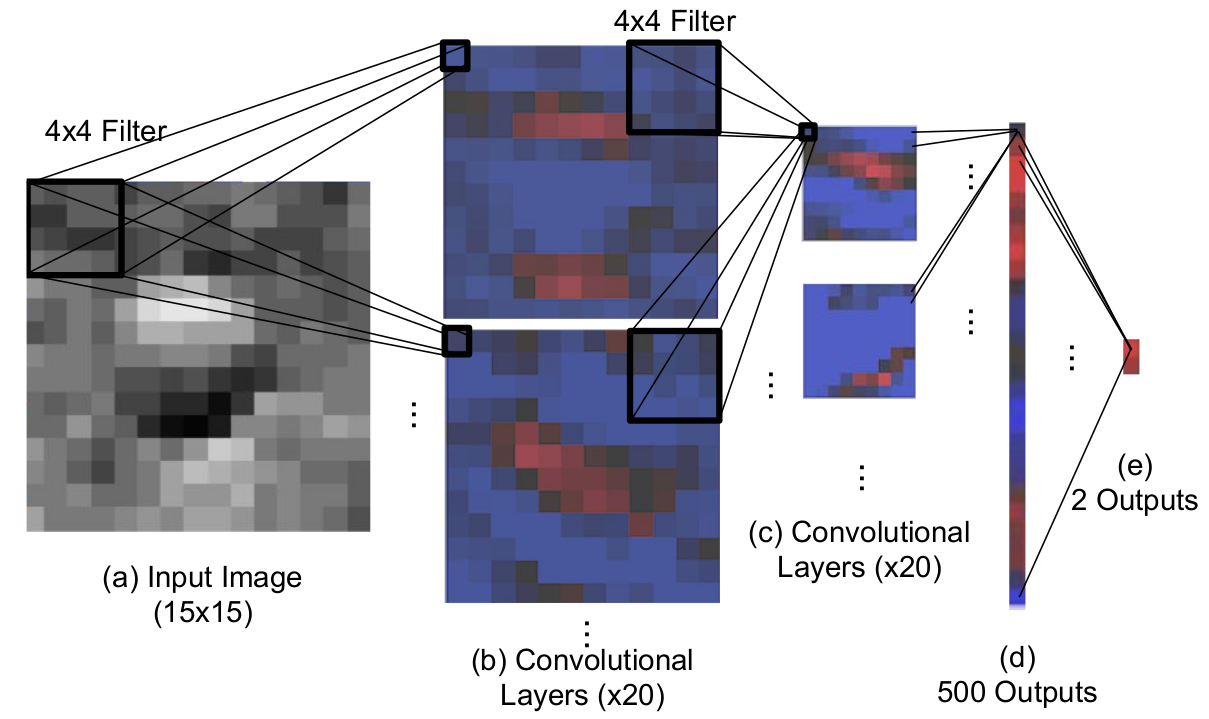
\includegraphics[width=.5\textwidth,keepaspectratio]{images/CLLD16_01.png}
	\caption{Die Architektur des Netzwerkes, aus \cite{cohen_16}}
	\label{fig:CLLD16_01}
\end{figure}

Der Unterschied zwischen dieser Methode und dem hier vorgestellten Ansatz besteht darin, dass in dieser Methode nur bewertet wird, ob Kraterkandidaten wirkliche Krater sind oder nicht, während hier ein Ansatz entwickelt wird, der aus einer kompletten Aufnahme der Marsoberfläche einzelne Krater(kandidaten) erkennt.

\subsection{Vergleich der Methoden}
\label{ssec:vergleich}

Die drei genannten Algorithmen (Urbach '09 \cite{urbach_stepinski_2009}, Bandeira '10 \cite{bandeira_10} und Cohen '16 \cite{cohen_16}) wurden alle auf der selben Aufnahme der HRSC angewandt. Eine genauere Beschreibung und der Vergleich anhand dieser Aufnahme findet sich in Abschnitt~\ref{sec:vergleich}.

